\documentclass[11pt]{article}
% ******************************************************************
% ******************* PHYSICS HEADER ************************
% ***********************************************************
% Version 2 

\usepackage{amsmath}	% AMS Math Package
\usepackage{amsthm}		% Theorem Formatting
\usepackage{amssymb}	% Math symbols such as \mathbb
\usepackage{graphicx} 	% Allows for eps images
\usepackage{multicol} 	% Allows for multiple columns

 % Sets margins and page size
\usepackage[dvips,letterpaper,margin=0.75in,bottom=0.75in,headheight=15pt]{geometry}

\pagestyle{empty} 		% Removes page numbers
\makeatletter	 		% Need for anything that contains an @ command 
\renewcommand{\maketitle} % Redefine maketitle to conserve space
{ \begingroup \vskip 10pt \begin{center} \large {\bf \@title}
	\vskip 10pt \large \@author \hskip 20pt \@date \end{center}
  \vskip 10pt \endgroup \setcounter{footnote}{0} }
\makeatother 			% End of region containing @ commands

\renewcommand{\labelenumi}{(\alph{enumi})} 					% Use letters for enumerate
% \DeclareMathOperator{\Sample}{Sample}
\let\vaccent=\v 											% rename builtin command \v{} to \vaccent{}
\renewcommand{\v}[1]{\ensuremath{\mathbf{#1}}} 				% for vectors
\newcommand{\gv}[1]{\ensuremath{\mbox{\boldmath$ #1 $}}}	% for vectors of Greek letters
\newcommand{\uv}[1]{\ensuremath{\mathbf{\hat{#1}}}} 		% for unit vector
\newcommand{\abs}[1]{\left| #1 \right|} 					% for absolute value
\newcommand{\avg}[1]{\left< #1 \right>} 					% for average
\let\underdot=\d 											% rename builtin command \d{} to \underdot{}
\renewcommand{\d}[2]{\frac{d #1}{d #2}} 					% for derivatives
\newcommand{\dd}[2]{\frac{d^2 #1}{d #2^2}} 					% for double derivatives
\newcommand{\pd}[2]{\frac{\partial #1}{\partial #2}} 		% for partial derivatives
\newcommand{\pdd}[2]{\frac{\partial^2 #1}{\partial #2^2}} 	% for double partial derivatives
% for partial cross derivatives
\newcommand{\pdc}[3]{\frac{\partial^2 #1}{\partial #2\partial #3}}

\newcommand{\ket}[1]{\left| #1 \right>} 				% for Dirac bras
\newcommand{\bra}[1]{\left< #1 \right|} 				% for Dirac kets
\newcommand{\braket}[2]{\left< #1 \vphantom{#2} \right|
 \left. #2 \vphantom{#1} \right>} 						% for Dirac brackets
\newcommand{\matrixel}[3]{\left< #1 \vphantom{#2#3} \right|
 #2 \left| #3 \vphantom{#1#2} \right>} 					% for Dirac matrix elements
\newcommand{\grad}[1]{\gv{\nabla} #1} 					% for gradient
\let\divsymb=\div 										% rename builtin command \div to \divsymb
\renewcommand{\div}[1]{\gv{\nabla} \cdot #1} 			% for divergence
\newcommand{\curl}[1]{\gv{\nabla} \times #1} 			% for curl
\let\baraccent=\= 										% rename builtin command \= to \baraccent
\renewcommand{\=}[1]{\stackrel{#1}{=}} 					% for putting numbers above =

\newtheorem{prop}{Proposition}
\newtheorem{thm}{Theorem}[section]
\newtheorem{lem}[thm]{Lemma}
\theoremstyle{definition}
\newtheorem{dfn}{Definition}
\theoremstyle{remark}
\newtheorem*{rmk}{Remark}

% ***********************************************************
% ********************** END HEADER *************************
% ***********************************************************

\title{Argo Float Profile Cycle Timing - MEDS DAC}
\author{Christopher Gordon}
\date{\today}

\begin{document}
	% creates the title/author/date
	\maketitle

    Following the Argo Science Team meeting, the Argo Canada team began changing the timing parameters for our NKE ARVOR floats. This includes already operating floats, which we changed via over-air messages to the float. The default settings for NKE ARVOR floats are to profile every 240 hours (10 days), and for the first profile to surface at 06:00 UTC, therefore most NKE floats surface at 06:00 UTC every 10 days. This change is motivated by work presented by Ken Johnson and Steve Riser at the AST meeting, and in \emph{Bif and Johnson (in prep.)} which shows that Argo floats can be used to estimate production as long as each float samples at diverse times of day. 

    \section{NKE Parameter Changes}

    Before implementing any parameter changes, we simulated the surfacing time for several different cycle periods. Figure 1 shows the surfacing times for each cycle number for the first year and a corresponding histogram for how many profiles per hour of the day that float would produce in its lifetime (assumed 5 years) for cycle periods of 245~hr (A, B), 246~hr (C, D) and 247~hr (E, F). The plot for 10 days + 6 hours (C, D, 246~hr) shows that offsetting the float cycle period by a factor of 24 does not accomplish the goal of having well distributed samples over a diurnal cycle. We chose to use a cycle time of 245~hr for our floats as it was the cycle period closest to the traditional 10-day Argo cycle that provided an even distribution across all times of day. 

    % time of day for each cycle time figure
    \begin{figure}[ht]
        \centering
        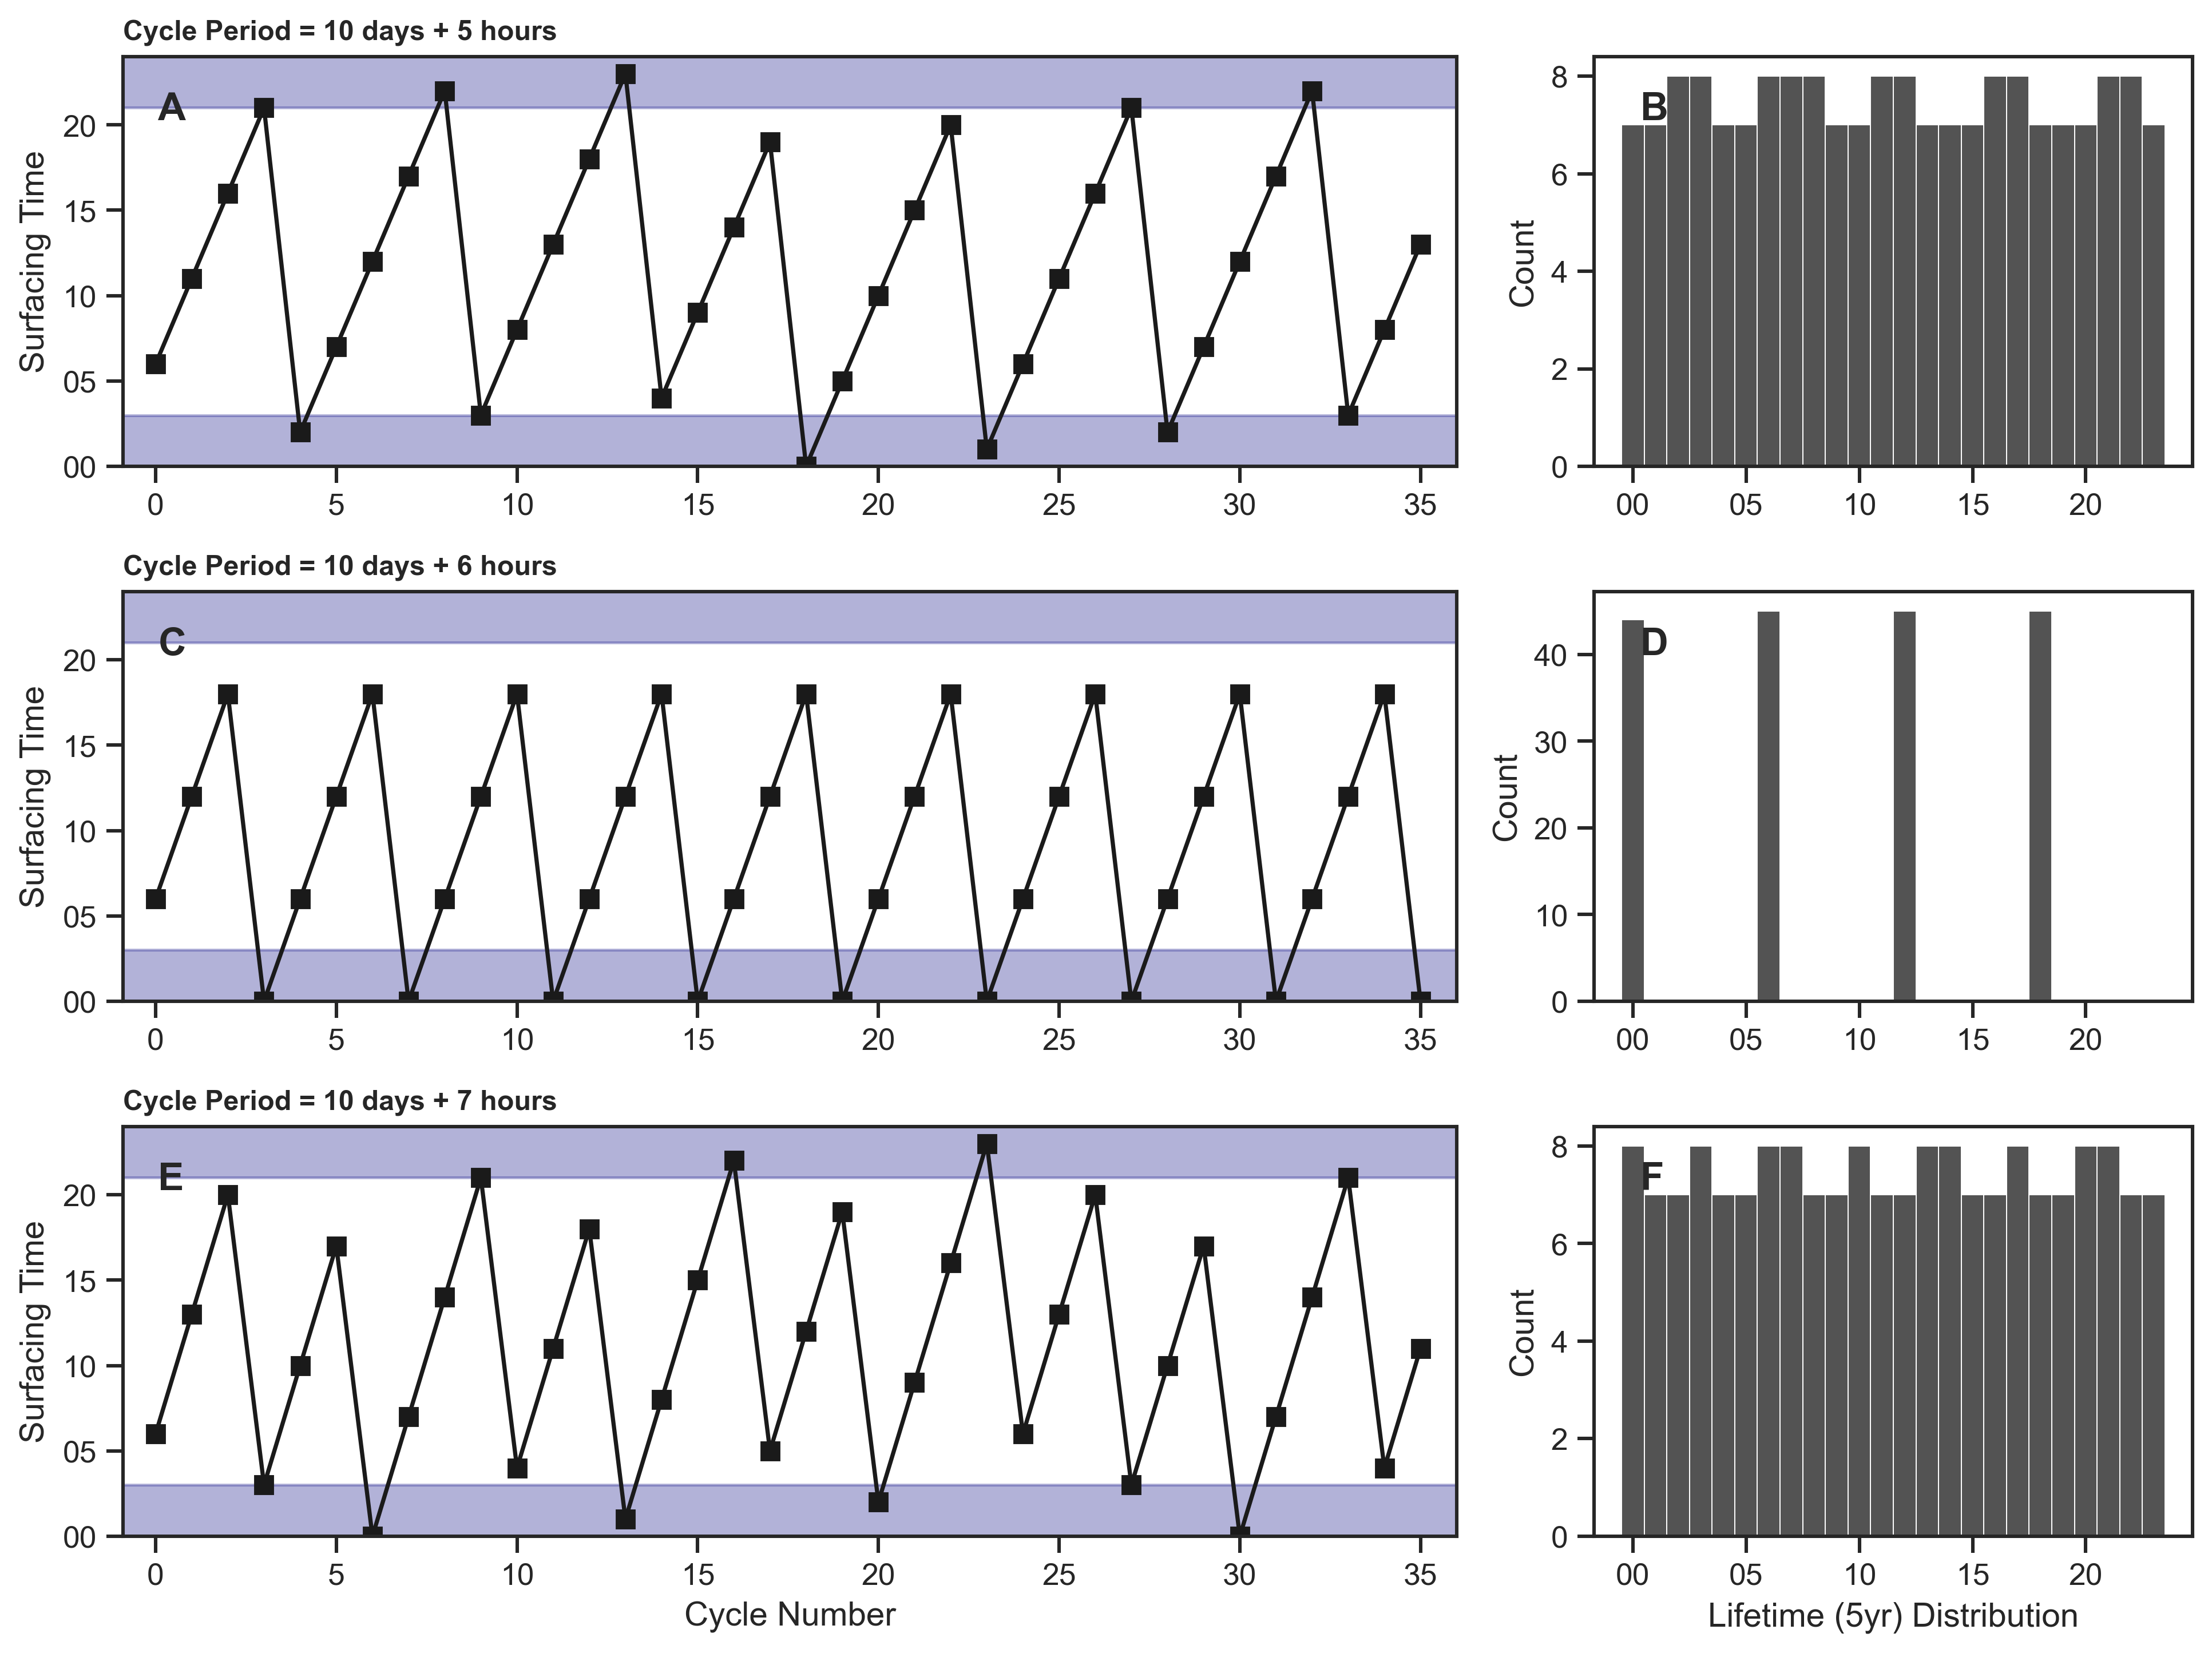
\includegraphics[width=0.8\textwidth]{../figures/profile_time_of_day_1yr_updated.png}
        \caption{Simulation of different float cycle surfacing times and histograms of number of profiles in each hour of the day for periods of (A, B) 10 days + 5 hours, (C, D) 10 days + 6 hours, and (E, F) 10 days + 7 hours.}
    \end{figure}

    Cycle times of 241~hr, 251~hr, and 243~hr were also considered (Figure 2). For the 10 days + 1 hour cycle period (241~hr), it would take 24 cycles ($\sim$2/3 of a year) to populate a diurnal timeseries, and seasonal bias could be introduced. For example, if the float were deployed in the summer with a 6AM local inital surfacing time, the first 4-8 points of the diurnal timeseries would be from the summer, while the afternoon and evening part of the diurnal timeseries would all be populated during the winter. Without proper investigation it is hard to estimate what type of biases this seasonality might introduce, however we felt it best to avoid the situation completely by choosing the 5~hr offset. 

    % put the 1/11/13 hr plot here
    \begin{figure}[ht]
        \centering
        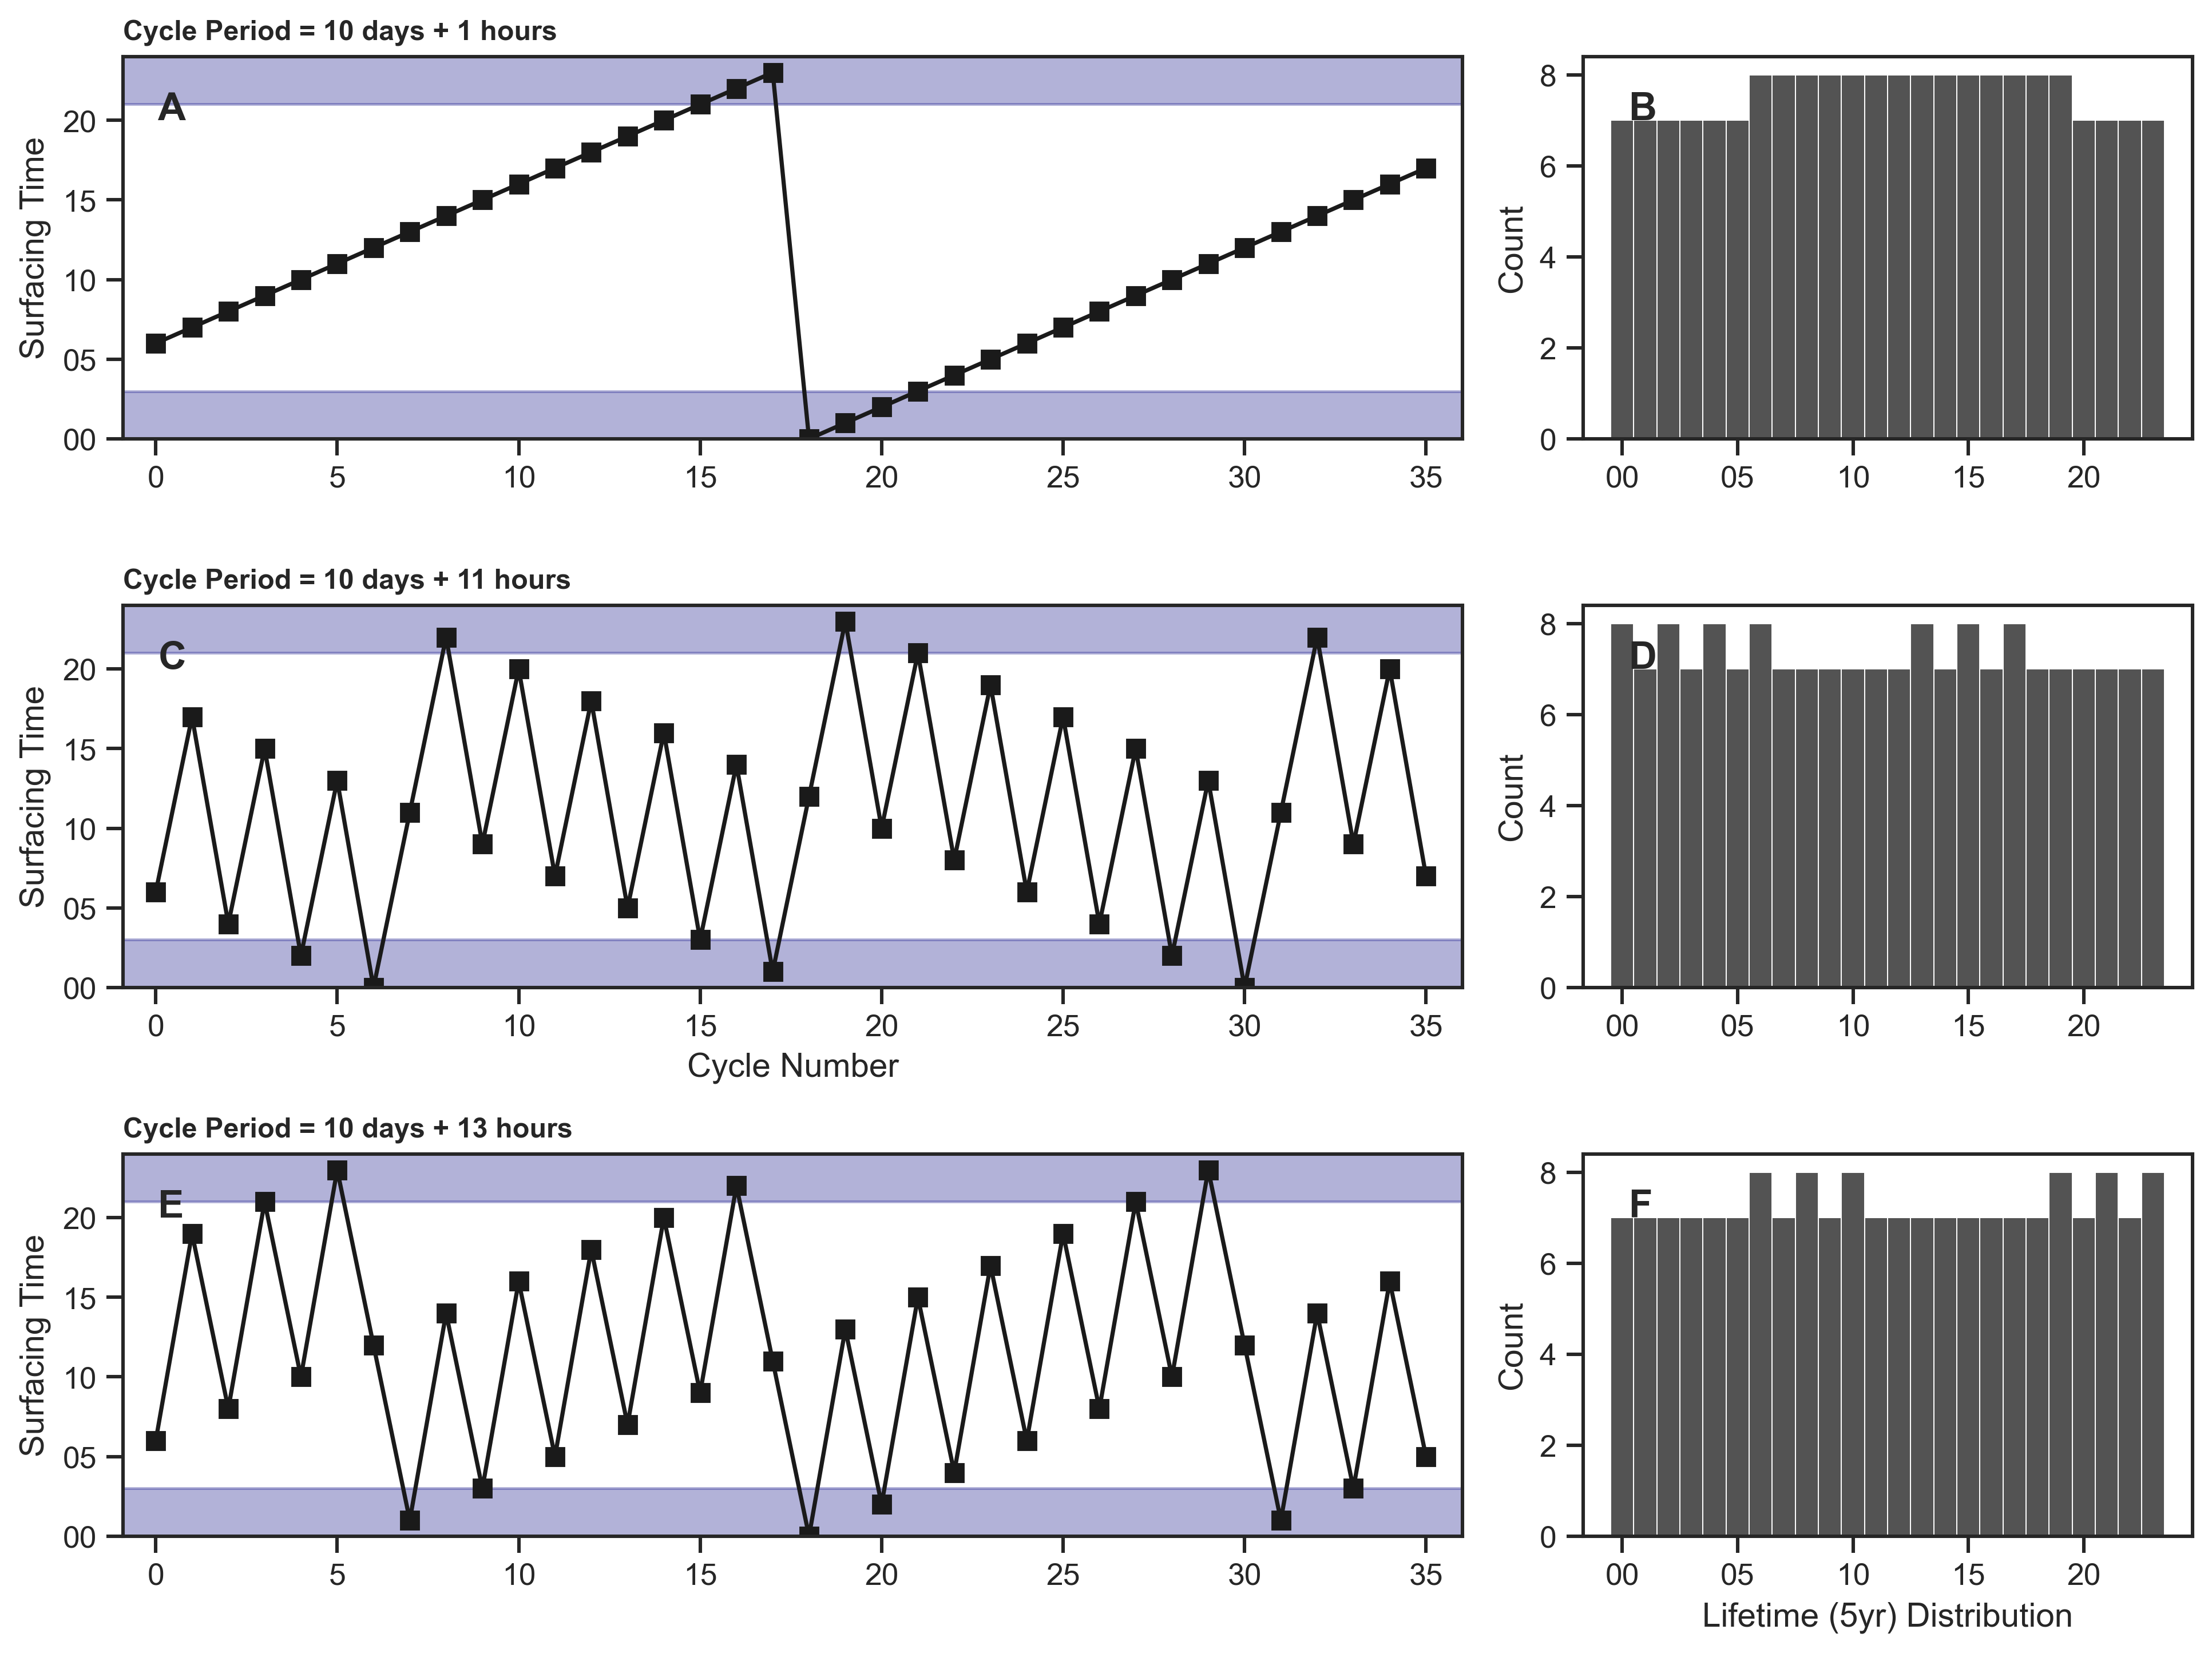
\includegraphics[width=0.8\textwidth]{../figures/profile_time_of_day_near12hr_1yr_updated.png}
        \caption{Alternate simulated float cycle surfacing times and corresponding histograms for periods of (A, B) 10 days + 1 hour (C, D) 10 days + 11 hours and (E, F) 10 days + 13 hours.}
    \end{figure}

    For the 10 days + 11 hour and + 13 hour cycle periods, although they would not suffer from the same seasonal bias issue described above, the 5 hour offset still was the better choice to fill in the diurnal timeseries and sample at pseudo-random times of day.

    For an NKE float, the parameters that adjusts the float cycle time are MC2 and MC3, depending on the configuration of some other parameters. The cycle time can be changed by the commands \verb|!MC 2 245| and \verb|!MC 3 245|. 

    \section{Vertical Resolution}

    The default resolution for NKE floats is also relatively low, sampling in 1~dbar bins from the surface to 10~dbar, in 10~dbar bins from 10~dbar to 200~dbar, and then in 25~dbar bins below 200~dbar. This results in only about 100 points for each profile. 

    The Argo Canada team adjusted our floats to the maximum resolution we could achieve for the data plans used for each float. This may vary from DAC to DAC depending on Iridium costs, but is included here as a note that these are other default parameters a DAC may want to adjust. Figure 3 shows profiles from before and after this parameter change for float 4902540. The new resolution samples at 1~dbar bins from the surface to 475~dbar, 5~dbar bins from 475~dbar to 1000~dbar, and 10~dbar bins below 1000~dbar. This results in a total of about 680 points, almost 7x the resolution of the default parameters. 

    % placeholder figure, make upper/lower be before/after, also add subfigure labels
    \begin{figure}[ht]
        \centering
        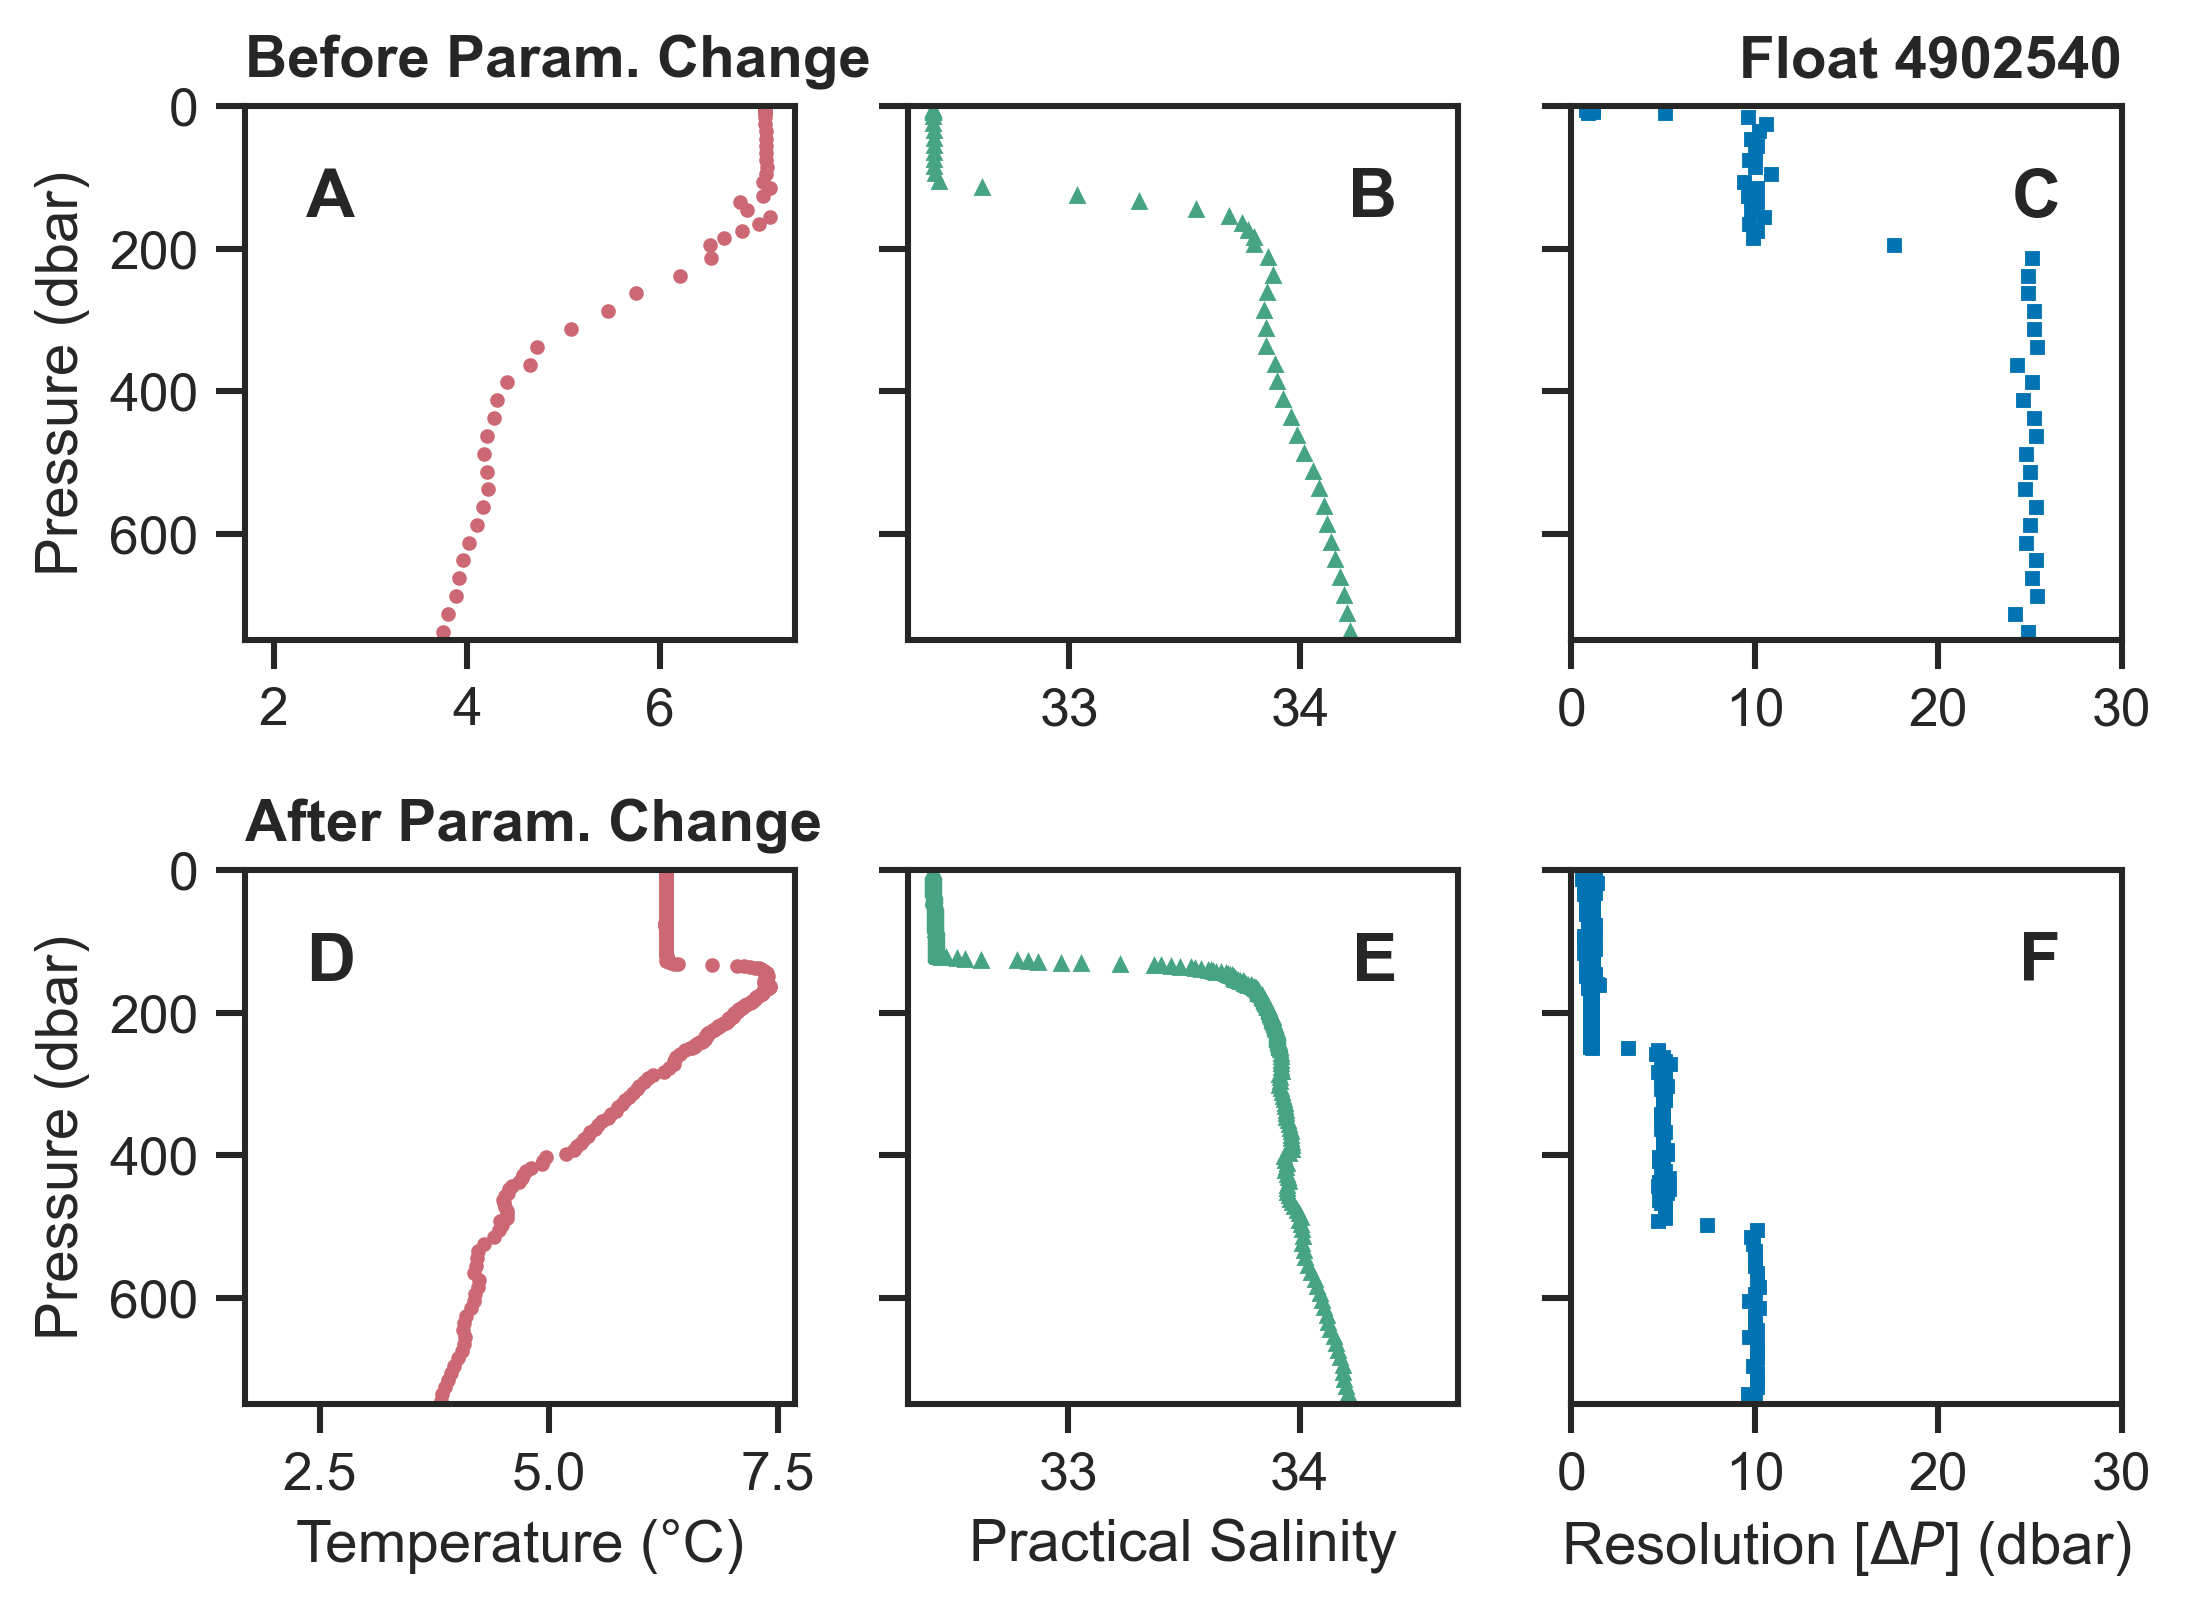
\includegraphics[width=0.8\textwidth]{../figures/meds_before_after_res_results.png}
        \caption{Profiles for before (A-C) and after (D-F) vertical resolution parameter changes for (A, D) temperature (B, E) salinity, and (C, F) the change in pressure between adjacent points.}
    \end{figure}

\end{document}